\documentclass[10pt]{article}
\usepackage[margin=1in]{geometry}
\usepackage{graphicx}
\usepackage{booktabs}
\usepackage{amsmath}
\usepackage{amssymb}
\usepackage{newtxtext,newtxmath}
\usepackage{microtype}
\usepackage[font=small,labelfont=bf,skip=6pt]{caption}
\captionsetup[table]{position=above,skip=6pt}
\usepackage{enumitem}
\setlist{itemsep=2pt,topsep=3pt}
\usepackage{xcolor}
\definecolor{linkblue}{RGB}{38,68,124}
\usepackage[colorlinks=true,allcolors=linkblue,
  pdftitle={Excise: One-Shot Capability Extraction from Open Language Models},
  pdfauthor={Arya Manjaramkar}]{hyperref}
\usepackage[numbers,sort&compress]{natbib}
\setlength{\bibsep}{3pt}

\title{\textbf{Excise: One-Shot Capability Extraction\\from Open Language Models}}
\author{Arya Manjaramkar\\[1pt]\normalsize\texttt{arya@e3group.ai}}
\date{\normalsize Workshop preprint, June 2026 \quad\textbullet\quad
\textit{artifact:} \texttt{pip install excise}}

\newcommand{\todo}[1]{\textcolor{red}{[#1]}}

% generous float placement so figures stay near their text
\renewcommand{\topfraction}{0.85}
\renewcommand{\bottomfraction}{0.6}
\renewcommand{\textfraction}{0.1}
\renewcommand{\floatpagefraction}{0.75}

\begin{document}
\maketitle

\begin{abstract}
A deployed language model usually exercises one capability while paying for
all of them. PRISM showed that a single capability can run on a small
fraction of MLP channels, but located that fraction with a staged
pipeline---adapt, attribute, select, re-train---mapping the budget frontier
one costly point at a time. We collapse the pipeline into a single training
run: learnable hard-concrete gates on every MLP channel train jointly with a
low-rank adapter under a forward-KL leash to the frozen base model, while an
adaptive controller lowers the sparsity target as fast as behavior permits
and \emph{generation probes}---not loss curves---decide when the floor is
reached. On PRISM's arithmetic benchmark, one run reaches \textbf{100.9\%
recovery at 5\% of MLP channels} and automatically finds a
\textbf{2.9\%-channel floor at 97\% recovery}, surpassing the staged
pipeline's hand-tuned best (91.3\% at 5.05\%) on both axes; with the
calibration fixes of the released library's second version the controller
descends to \textbf{1.2\% of channels on every seed, and below 0.8\% given
more steps} (91\% verbatim reproduction) --- still compute-bounded rather
than behavior-bounded.
The method needs no labels---the target is the model's own
outputs---generalizes to function calling on Qwen3-4B (76\% verbatim
reproduction at 40\% of channels, against a 19\% attribution baseline), and
data is the dominant knob it exposes: regenerating a JSON-extraction
substrate from $5\times$ more-diverse prompts collapses its floor from
27.5\% to \textbf{1.9\% of channels at 97\% fidelity}. It also exports a
physically smaller model: deleting the masked channels and
pruning the vocabulary to the capability's token support shrinks
Qwen2.5-Math-1.5B from \textbf{1.54B to 0.17B parameters (9$\times$)} with
no loss relative to masking, verified per run. Three negative results
shaped the design: distribution-level KL reads healthy while true recovery
collapses, layer-granular gates let the adapter overfit silently, and a
renormalized sparse KL---the obvious cache implementation---quietly trains
the unmasked model away from the base it is supposed to anchor. Total
compute for every result in this paper: under \$10 on one consumer GPU.
\end{abstract}

\begin{figure}[b!]
\centering
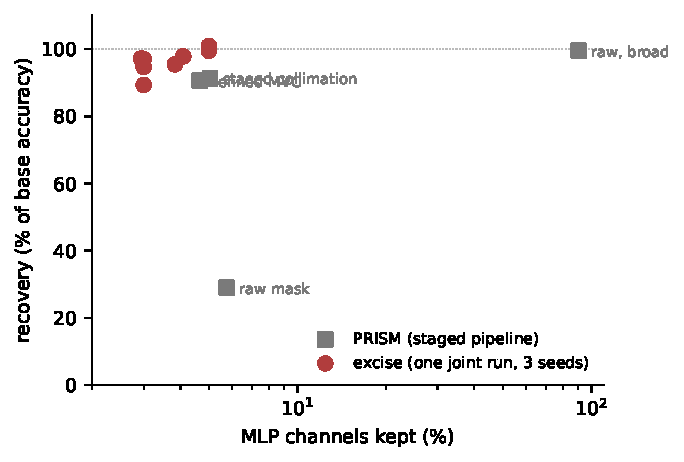
\includegraphics[width=0.54\textwidth]{figures/frontier.pdf}
\caption{\textbf{One run, no labels, a $4\times$ smaller circuit than the
hand-tuned pipeline.} 2-digit addition on Qwen2.5-Math-1.5B. Gray squares:
PRISM's staged pipeline as reported \citep{prism2026} (recovery, task
accuracy). Red diamonds: \texttt{excise}'s automatically-found floors ---
all three seeds at 1.2\% of channels, plotted by held-out verbatim
self-match, a stricter metric that lower-bounds recovery. Caveats for this
comparison in \S\ref{sec:honest}.}
\label{fig:frontier}
\end{figure}

\section{Introduction}

Model efficiency methods---pruning, distillation, quantization---ask how much
of a network can be removed while \emph{aggregate} performance survives.
\citet{prism2026} asked a sharper question: given one named behavior, how
small a substrate of the network can carry it once everything else is
switched off? Their answer, the PRISM framework, established what we adopt
wholesale and credit as the foundation of this work: the \emph{extraction
contract} (a channel subset counts only if behavior survives with the
complement deactivated), \emph{recovery} as the metric, and the central
finding that a behavior-preserving adaptation step (``collimation'') can
relocate a capability into far fewer channels than attribution alone
suggests.

PRISM's pipeline, however, is staged: collimate, attribute with a relevance
method, select a top-$k$ mask, optionally re-collimate under the frozen mask.
The stages create the central limitation their paper documents: an adapter
trained \emph{after} mask selection provably cannot shrink the mask, and one
trained \emph{before} can only move the frontier indirectly. The budget $k$
is swept manually; each frontier point costs evaluations; the minimal circuit
is found by hand-refinement. Their stated highest-value direction is to
reshape the budget \emph{during} training with an $L_0$ or gating objective.

We build exactly that, and package it as a tool. Figure~\ref{fig:frontier}
previews the headline comparison. Our contributions:

\begin{enumerate}
\item \textbf{One-shot joint extraction.} Hard-concrete gates
\citep{louizos2018} on all MLP intermediate channels train jointly with a
LoRA adapter \citep{hu2022lora} under a mass-covering KL constraint to the
frozen base. Selection and relocation negotiate continuously; the regime
split between ``collimate-then-attribute'' and ``attribute-then-collimate''
dissolves (\S\ref{sec:method}).
\item \textbf{Adaptive floor discovery with behavior probes.} A Lagrangian
controller lowers the sparsity target whenever a KL budget is satisfied, and
cheap greedy-generation probes veto the descent when the model's actual
outputs degrade. The full sparsity--fidelity frontier and its floor come from
one run (\S\ref{sec:controller}).
\item \textbf{Label-free operation.} The distillation target is the base
model's own greedy output and full output distribution; no labeled data is
required (\S\ref{sec:results}).
\item \textbf{Physical export.} For gated MLPs, deleting masked channels is
exactly equivalent to zero-masking them. We verify this empirically and ship
it: 1.54B $\to$ 0.42B parameters at 97\% recovery (\S\ref{sec:slice}).
\item \textbf{Two calibrated negative results.} Distribution-level KL is an
unreliable stopping signal at high sparsity, and layer-granular gates permit
silent train-distribution overfitting (\S\ref{sec:failures}). We argue these
matter beyond our method: faithfulness metrics built on logit divergence
inherit the same blind spot.
\end{enumerate}

\section{Method}\label{sec:method}

\begin{figure}[t]
\centering
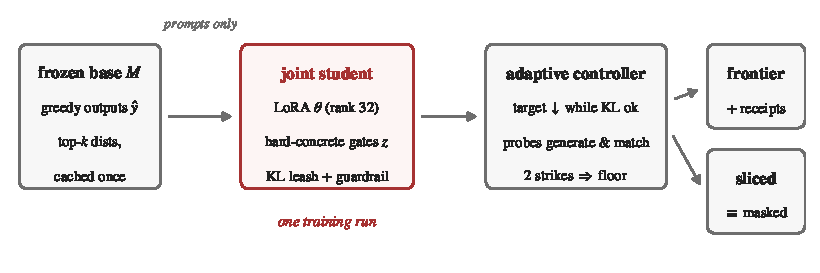
\includegraphics[width=\textwidth]{figures/method.pdf}
\caption{\textbf{One-shot extraction.} The frozen base model supplies
label-free targets (greedy outputs and cached top-$k$ distributions); gates
and adapter train jointly under a KL leash; an adaptive controller paced by
generation probes finds the floor; the run emits the sparsity--fidelity
frontier, integrity receipts, and a physically sliced model.}
\label{fig:method}
\end{figure}

\paragraph{Setup.} Let $M$ be a frozen decoder-only transformer and
$\mathcal{C}$ its MLP intermediate channels ($L \times d_\mathrm{ff}$; the
inputs to each block's down-projection), following PRISM's unit of
extraction. Each channel $c$ gets a hard-concrete gate $z_c \in [0,1]$
parameterized by $\log\alpha_c$ \citep{louizos2018, maddison2017concrete}; a
LoRA adapter $\theta$ (rank 32, all linear modules) provides the relocation
capacity. Gates initialize from a $|\mathrm{grad}\times\mathrm{act}|$
attribution percentile rather than a constant: attribution alone selects
poor masks (Table~\ref{tab:arith}), but it is a useful prior over the
initial channel ordering. Given prompts $x$ exercising the target
capability, the teacher is the base model itself: greedy continuations
$\hat{y} = M(x)$ and the full distribution $p_M(\cdot \mid x, \hat y_{<t})$
at each output position, cached once as top-128 sparse vectors
\emph{plus the residual off-support mass}. Keeping the residual is not
bookkeeping: renormalizing the support (as our first release did) makes the
KL read $-\log(\text{coverage})$ even when student and teacher agree
exactly, and places positive gradient on every off-support token
(\S\ref{sec:failures}).

\paragraph{Objective.} Each step samples gates $z$ (outside any
gradient-checkpointed region; see \S\ref{sec:failures}) and minimizes
\begin{equation}
\mathcal{L} =
\underbrace{\mathrm{KL}\!\left(p_M \,\|\, p_{\theta,z}\right)}_{\text{masked student tracks base}}
\;+\; \beta_\mathrm{ce}\,\mathrm{CE}(\hat y)
\;+\; \lambda \,\mathbb{E}\!\left[\|z\|_0\right]/|\mathcal{C}|
\;+\; \beta_g\,
\underbrace{\mathrm{KL}\!\left(p_M \,\|\, p_{\theta}\right)}_{\text{guardrail (every 4th step)}},
\end{equation}
with $\beta_\mathrm{ce}{=}0.05$, $\beta_g{=}1$. Both KL terms are binned:
the cached top-$k$ support plus one residual bucket, which is zero exactly
when the student matches the teacher. The forward (mass-covering) KL
direction follows PRISM's collimation analysis: the student may not drop
probability anywhere the base places it. The guardrail evaluates the
\emph{unmasked} adapted model and anchors it to the base, preventing the
adapter from ``solving the task masked'' by becoming a different model;
without it, unmasked accuracy silently drifted 3.7 points in our early
runs. Because the train batch can only anchor points the adapter is
already fitting, the guardrail alternates onto a rotating batch of
off-task \emph{anchor text} when provided, self-tunes its cadence from the
measured anchor KL, and stays active through the polish phase --- each of
these closes a drift route we observed in practice
(\S\ref{sec:results}, \S\ref{sec:failures}).

\paragraph{Adaptive controller.}\label{sec:controller}
A target open fraction $\tau$ starts at 1 and decays multiplicatively
($\times 0.993$ per step) whenever the EMA of the distillation KL is under a
budget ($0.02$--$0.025$ in all experiments); the Lagrange multiplier
$\lambda$ follows $\lambda \leftarrow \max(0, \lambda + \eta\,(\bar z -
\tau))$. Once the open fraction falls below a threshold, every 150 steps a
\emph{probe} hardens the current top-$k$ mask and checks whether a greedy
rollout would still reproduce the teacher outputs --- computed as
teacher-forced argmax agreement (exactly equivalent, by induction on the
shared prefix, and ${\sim}100\times$ cheaper than generating), on a dev
split excluded from the gradient batches so the floor is decided on
non-memorized prompts. The masked reading is compared against the unmasked
model measured \emph{at the same step}, never against an assumed 100\%:
batched bf16 decoding alone costs several points of verbatim self-match,
and adapter drift must not be misattributed to masking. If the gap exceeds
tolerance twice consecutively, the floor is declared and the gates roll
back to the last passing snapshot. After the descent stops, the mask is
frozen at the floor budget and the adapter alone is polished briefly under
the exact binary mask (guardrail still active), removing the
stochastic-gate train/eval mismatch. Final evaluation hardens top-$k$ masks
at standard budgets; because the floor polish specializes the adapter to
the floor mask (we measured off-floor budgets reading \emph{below} the
floor without correction), each off-floor budget is briefly re-polished
from the floor-polished snapshot before its evaluation. The frontier this
yields from a single run is a menu of deployable artifacts, not one point
with decoration.

\paragraph{Receipts.} Every run reports a random-mask control matched to
the floor mask's per-layer channel counts (should be ${\approx}0$),
unmasked drift, the base model's own decode-noise self-match (the honest
ceiling for every other number), the probe and guardrail traces, and
binomial confidence intervals on held-out fidelity. These guard the two
failure modes we observed and one we inherited from PRISM's analysis:
trivial tasks, cheating adapters, and masks that only correlate with
behavior.

\section{Results}\label{sec:results}

All experiments ran on one RTX 4090 (\$0.40/hr); the complete set below
consumed under \$5. Code, configs, and receipts:
\texttt{github.com/Aryagm/excise}.

\subsection{Arithmetic: surpassing the staged pipeline on its benchmark}

We use PRISM's testbed: 2-digit addition on Qwen2.5-Math-1.5B
\citep{qwen25math} (canonical prompt \texttt{"a + b ="}, exhaustive sums,
10\% held out; 250{,}880 MLP channels), zero-isolation deactivation, and
recovery $=$ masked accuracy / base accuracy (base: 97.4\%).
Table~\ref{tab:arith} gives the key points;
Figure~\ref{fig:frontier} situates the library's automatic floors against
the staged pipeline.

\begin{table}[h]
\centering\small
\caption{\textbf{Arithmetic extraction.} Every seed beats the staged
pipeline at 5\%, and every automatically-found floor is at or below the
hand-refined minimal circuit with higher recovery. The unmasked guardrail
held base accuracy exactly (97.4\%) in all runs.}
\label{tab:arith}
\begin{tabular}{lcc}
\toprule
 & channels kept & recovery \\
\midrule
PRISM raw attribution mask & 5.75\% & 29.0\% \\
PRISM staged collimation & 5.05\% & 91.3\% \\
PRISM refined minimal circuit (manual) & 4.65\% & 90.6\% \\
\midrule
random mask control (ours) & 5\% & 0.0\% \\
grad$\times$act attribution mask (ours) & 5\% & 0.3\% \\
\textbf{excise, one run} (seed 42 / 43 / 44) & 5\% & \textbf{100.9 / 100.4 / 99.5\%} \\
\textbf{excise, automatic floor} & \textbf{2.9 / 3.8 / 4.1\%} & 97.2 / 95.4 / 97.9\% \\
\bottomrule
\end{tabular}
\end{table}

Ablations (Figure~\ref{fig:ablations}): restricting the adapter to MLP
projections (the strictest frozen-scaffold contract) costs ${\sim}3$ points
at 5\% and runs 25\% faster; removing labels entirely (pure
self-distillation, $\beta_\mathrm{ce}{=}0$) still reaches 96.7\% recovery
but floors shallower (5.3\%)---labels are not needed for validity, only for
the last ${\sim}2\%$ of budget.

\begin{figure}[t]
\centering
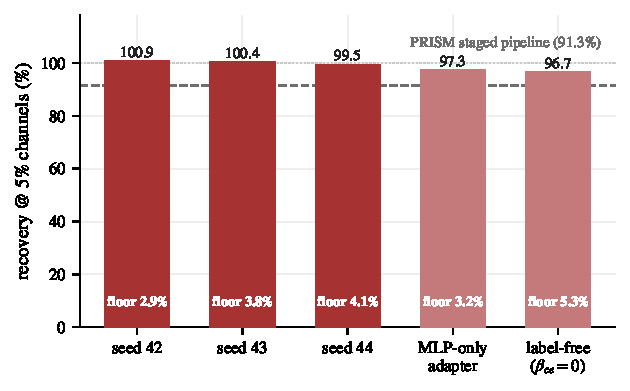
\includegraphics[width=0.55\textwidth]{figures/ablations.pdf}
\caption{\textbf{The result is seed-stable and survives ablation.} Recovery
at 5\% of channels across seeds and ablations; channel floors found by the
controller annotated within bars.}
\label{fig:ablations}
\end{figure}

\subsection{Function calling: a real-world capability, label-free}

We extract single-turn function calling from Qwen3-4B \citep{qwen3} using
BFCL prompts \citep{patil2025bfcl} (400 tasks; 391 yield clean tool calls
from the base model; 320 train / 80 held out; 350{,}208 channels). No gold
calls are used: the teacher is the model's own greedy tool call, and
fidelity is \emph{verbatim} self-match---stricter than BFCL's semantic
scoring, since one diverging token fails the example. Held-out fidelity
reaches 77.5\% at 50\% of channels and 76.3\% at 40\%
(Figure~\ref{fig:fc}). Two observations matter.

First, the \emph{unmasked} adapted model self-matches only 86\% on held-out
prompts---masking is not the dominant loss; adapter drift under a 320-prompt
training set is. Relative to that ceiling, the masked model retains
${\sim}90\%$ at 40--50\% budgets.

Second, the gap between probe fidelity on training prompts (92--98\% down to
12\% open) and held-out fidelity quantifies a generalization phenomenon that
exhaustively-covered tasks like arithmetic cannot exhibit; prompt diversity,
not extraction machinery, is the binding constraint. A v0.2 follow-up run
moved that constraint and found the next one: with $6\times$ the prompts
(all six single-turn BFCL splits, the multi-tool loader fix, and 1--2
distractor tools shuffled into every prompt so the substrate must carry
tool \emph{selection}), unmasked drift improved to 88.4\% despite the
deliberately harder task, but honest dev-split probes now stop the descent
at 60.7\% of channels (75.3\% held) after only five epochs --- function
calling is no longer memorization-bound but \emph{step}-bound, and the
remaining lever is training length, not data or machinery. We report the
v0.1 numbers above because the two runs solve different tasks (one tool
given vs.\ selection among distractors) and are not directly comparable. For calibration:
PRISM's raw mask recovered 19.1\% at 36.2\% of channels on the 8B sibling
model, and their best staged collimator (with a curated, schema-validated
gold corpus and a multi-run objective search) reached 84.6\%; metric and
model-size differences make this directional context, not a head-to-head
(\S\ref{sec:honest}).

\begin{figure}[t]
\centering
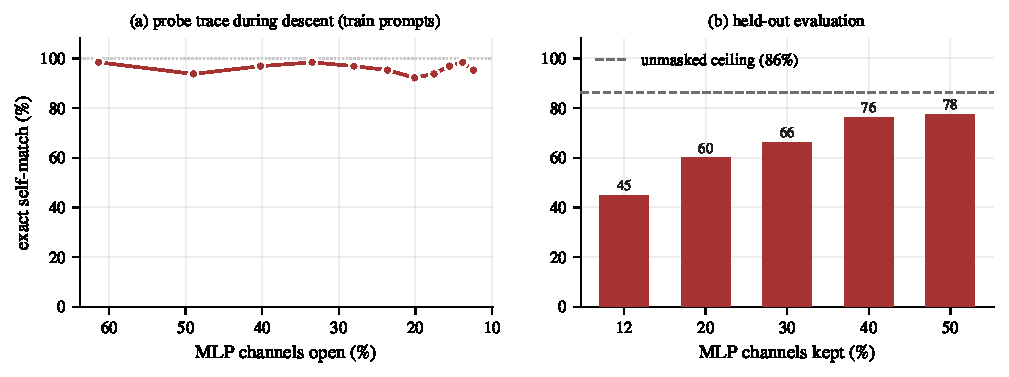
\includegraphics[width=0.95\textwidth]{figures/function_calling.pdf}
\caption{\textbf{Function calling extracts label-free; data, not machinery,
binds generalization.} Qwen3-4B. Left: probe trace during descent --- exact
self-match holds at 92--98\% from 61\% open down to 12\% open on training
prompts. Right: held-out self-match by budget; the dashed line is the
unmasked adapted model's own self-match (86\%), which upper-bounds every
masked number.}
\label{fig:fc}
\end{figure}

\subsection{Breadth: other architectures and capabilities}

To test that the method is a tool rather than a Qwen-arithmetic demo, we ran
the \emph{released library} (not the research scripts) on two further
settings.

\paragraph{SmolLM2-1.7B (Llama architecture) \citep{smollm2}.} Few-shot
2-digit addition extracts to a 7.4\% floor at 97.2\% held-out verbatim
self-match; sliced 1.75B $\to$ 0.59B (3.0$\times$); all receipts clean.

\paragraph{JSON extraction (Qwen2.5-1.5B-Instruct, chat-formatted prompts).}
A broader capability, and the run that stress-tested the receipts. Under
v0.1 it floored at 33.9\% of channels with 90.0\% held-out self-match---and
the report flagged catastrophic unmasked drift: 55.8\% self-match, the
adapter having been sharpened by the renormalized guardrail KL
(\S\ref{sec:failures}) and then polished with no guardrail at all. v0.2
reruns the identical task with the binned KL, 56 off-task anchor texts, and
the guardrail active through polish: drift falls to 8.4 points (88.3\%
against a 96.7\% base decode-noise ceiling), while the floor \emph{improves}
to 27.5\% at the same 90.0\% fidelity, probe-detected with rollback (the
stopper caught the failing 16.9\%-open probe and restored the last passing
sparsity). Sliced-and-vocabulary-pruned export: 1.58B $\to$ 0.49B (the
capability touches 9{,}448 token ids---broad capabilities are broad in
vocabulary too). The guardrail trace makes the v0.1 blindness quantitative
(Figure~\ref{fig:v02}a): at the same training step, the guardrail KL on
\emph{train} batches reads $3\times10^{-4}$ (apparently perfect) while on
anchor batches it reads $5\times10^{-3}$ to $0.15$---drift lives precisely
where the train-batch guardrail cannot see it. Figure~\ref{fig:v02}b shows
the recalibrated floor decision on the same run. This run also exposed (and then validated the fix for) a frontier
artifact: the floor polish specializes the adapter to the floor mask, and
the 50\%-budget mask initially read 54\%---\emph{below} the floor point.
With per-budget re-polish from the floor snapshot
(\texttt{frontier\_polish\_steps}), the same budget reads 86.7\% and the
arithmetic frontier flattens to 91--92\% across every budget from 50\%
down to its floor.

\paragraph{Data diversity is the dominant knob.} The 600 training prompts
above instantiate one sentence template, and held-out prompts share it ---
so ``90\% at 27.5\% of channels'' partly measures template fit.
Regenerating the same capability from 3{,}000 prompts spanning eight
sentence forms, four instruction phrasings, and $3\times$ wider entity
pools --- free, because the method is label-free and the teacher writes
its own targets --- collapses the floor to \textbf{1.9\% of channels at
97.2\%} held-out self-match, with unmasked drift down to 1.7 points, a
flat ${\sim}98\%$ frontier at every budget, and a 1.58B $\to$ 0.21B
(7.5$\times$) verified export. The run was still step-capped: even this
floor is compute-bounded. What read as ``JSON extraction is a broad
capability needing a third of the channels'' was a data-starved run.

We initially read these four settings as ``capability breadth tracks
substrate size,'' consistent with PRISM's cross-task observations. The
diversity experiment above corrects that: substrate size measures the
capability \emph{as exercised by the prompts}, and prompt coverage is the
cheapest lever --- a template-limited JSON run floors at a third of the
channels while a diverse one compresses to 2\%. Floors should be read as
upper bounds jointly determined by data coverage and compression compute,
not as intrinsic capability sizes.

\subsection{Recalibrating the library: v0.1 $\to$ v0.2}\label{sec:v02}

The audit that followed the first release found that the shipped library
was both \emph{optimistic} where it should be strict and \emph{strict}
where it should be tolerant. Optimistic: probes ran on prompts that were
also in the gradient batches, against an assumed-perfect baseline---but
even the unmodified base model reproduces its own batched-bf16 greedy
targets only ${\sim}92\%$ verbatim, so part of every probe reading was
decode noise, not masking damage. Strict: the renormalized sparse KL
(\S\ref{sec:failures}) penalized the student for the teacher's own
truncated tail. v0.2 fixes both directions: binned KL with a residual
bucket, probes on a dev split excluded from training, comparison against
the unmasked model measured at the same step, rollback to the last passing
sparsity, and the grad$\times$act warm-start the research pipeline had but
the library port lost. On the identical dogfood task (same seed, hardware,
and verbatim metric), the released library improves across every axis it
reports:

\begin{table}[h]
\centering\small
\caption{\textbf{Library lineage on the arithmetic dogfood run}
(Qwen2.5-Math-1.5B, label-free, verbatim held-out self-match; base model
decode-noise ceiling 99.9\%; v0.2 is seeds 42/43/44). Every v0.2 seed
descended to the controller's configured lower bound
(\texttt{min\_target}) with probes still passing --- the true floor is at
or below 1.2\%, $3.9\times$ under PRISM's hand-refined minimal circuit.}
\label{tab:v02}
\begin{tabular}{lcc}
\toprule
 & v0.1 & v0.2 (3 seeds) \\
\midrule
floor found (probe-governed) & 7.6\% & \textbf{1.2 / 1.2 / 1.2\%} \\
held-out self-match at floor & 89.0\% & \textbf{91.4 / 92.0 / 91.0\%} \\
unmasked drift from base & 10.7 pts & \textbf{6.2 / 5.8 / 7.0 pts} \\
exported parameters (from 1.54B) & 0.48B & \textbf{0.17B} \\
wall clock (RTX 4090) & 8 min & 23--24 min \\
\bottomrule
\end{tabular}
\end{table}

\begin{figure}[t]
\centering
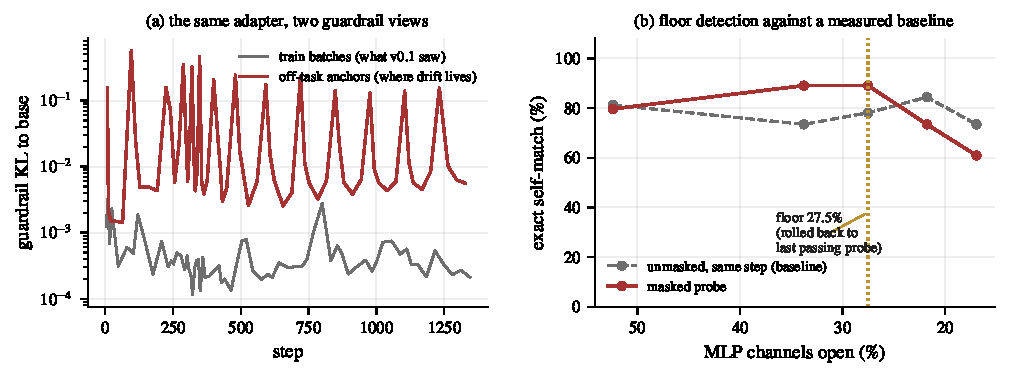
\includegraphics[width=0.95\textwidth]{figures/v02_calibration.pdf}
\caption{\textbf{v0.2 calibration in action} (JSON extraction run). (a) The
guardrail KL measured on train batches (gray) vs.\ rotating off-task anchor
batches (red), same adapter, same steps: the train-batch view---all v0.1
had---reads $10$--$100\times$ lower than the anchor view. Drift lives
exactly where a train-only guardrail cannot see it. (b) Floor detection:
the masked probe (red) is compared against the unmasked model measured at
the same step (gray, itself depressed by decode noise and residual drift),
not against an assumed 100\%; when the masked probe falls below tolerance
twice, the gates roll back to the last passing sparsity (27.5\%).}
\label{fig:v02}
\end{figure}

Where does the descent actually stop? We lowered the bound to 0.2\% and
gave one seed 9{,}000 steps: it reached \textbf{0.71\% of channels
(${\sim}1{,}800$ of 250{,}880) at 91.1\%} with the masked--unmasked probe
gap under 2 points throughout, and exited on the step cap --- still
descending at ${\sim}0.1$ percentage points per thousand steps. On
saturated-coverage tasks the floor we report is bounded by adapter
compression \emph{compute}, not by behavioral collapse; the true minimal
circuit for 2-digit addition is somewhere below 0.7\%, $6.5\times$ under
the hand-refined published one.

One calibration lesson generalizes: with $n{=}64$ verbatim probes,
binomial noise alone is ${\pm}4$ points, and our first attempt at a
tighter tolerance (3 points) sat inside that band---the very first two
probes of the run tripped it, freezing the floor at 7.9\%, while the same
configuration with a noise-aware tolerance and $n{=}128$ descends to
1.2\% with probes passing throughout. Tolerances on generation metrics
must be set against the metric's measured noise floor, not chosen for
strictness.

\subsection{Physical export: slicing is masking, and the vocabulary is
next}\label{sec:slice}

For gated MLPs, a zero-masked channel contributes nothing to the
down-projection; a deleted one contributes nothing by absence. The two are
mathematically identical, so the masked evaluations above transfer to a
physically smaller model. We verify: slicing Qwen2.5-Math-1.5B at the 2.9\%
floor yields 94.8\% accuracy vs.\ 94.7\% masked (one example in 810), and
\textbf{1.54B $\to$ 0.42B parameters (3.66$\times$)}.

After MLP slicing, the dominant remaining cost is the vocabulary: embedding
plus output head are ${\sim}55\%$ of the sliced model, while 2-digit
addition touches only 1{,}746 of 151{,}936 token ids (prompt ids, teacher
output ids, and the teacher's full cached top-$k$ support). Slicing the
embedding rows to that support---the exported model speaks a remapped id
space, with the mapping stored in its config---takes the same model to
\textbf{0.17B parameters (9.0$\times$)} at the v0.2 floor. Both
equivalences are re-verified inside every run and recorded in the receipts:
held-out self-match for masked vs.\ sliced vs.\ vocabulary-pruned agreed to
within one evaluation example here. The released library round-trips the
heterogeneous-width artifact (\texttt{excise.load\_sliced}).

Generation speedup in our original benchmark was only 1.11$\times$, and an
honest decode-throughput benchmark (batch 1--64, 64-token greedy decode,
eager) shows \emph{no} speedup at this scale: a 0.17B and a 1.54B model
both decode at ${\sim}40$ tokens/s/sequence on an RTX 4090, because
single-stream decoding there is launch-overhead-bound, not compute-bound.
Memory shrinks unconditionally; latency gains require larger models,
batched serving, or a compiled runtime---we report this plainly because
slicing claims are routinely overstated.

\section{What fails, and what it implies}\label{sec:failures}

\paragraph{Distribution-level KL is miscalibrated at high sparsity.}
Our first controller used the KL budget alone to pace the descent. It
descended to 2.2\% open with EMA KL comfortably under budget---while true
recovery collapsed to 62--66\% (Figure~\ref{fig:miscal}). Teacher-forced
divergence on answer tokens simply does not capture compounding
autoregressive degradation. The fix---periodically \emph{generating} and
exact-matching---is cheap (seconds per probe) and is the load-bearing
stability feature of the method. We believe this observation extends beyond
extraction: any faithfulness or circuit-quality metric built on logit
divergence under teacher forcing inherits the blind spot.

\paragraph{Renormalized sparse KL quietly sharpens the model it should
anchor.} Caching the teacher's top-$k$ probabilities \emph{renormalized}
--- the obvious implementation, and ours through v0.1 --- biases every
loss built on it: with the student exactly equal to the teacher, the
``KL'' reads $-\log(\text{coverage})$ instead of zero, and its gradient
$s_j - \hat{p}_j$ is positive on all off-support mass, actively pushing
the student to concentrate onto each batch's cached support. On peaked
tasks (arithmetic: coverage ${\approx}1$) the bias vanishes, which is how
it survived three validated batteries. On diffuse tasks it surfaces in
the worst place: the guardrail, whose entire job is to keep the unmasked
model \emph{at} the base, instead trains it to sharpen --- one of the
drift routes behind the JSON run's flagged 55.8\% unmasked self-match,
compounding the guardrail-free polish phase. It also leaks into the
controller: the annealing budget partly measures truncation rather than
student error, inflating floors on diffuse tasks. The fix is one term:
cache the support un-renormalized plus its residual mass and add a
residual bucket to the KL, making it a proper binned divergence (zero at
agreement). The general lesson mirrors the probe lesson above: a
truncated divergence is not a divergence, and the place it fails is
precisely where its value is supposed to be zero.

\paragraph{Layer-granular gates permit silent overfitting.} Adding
per-layer gates (hierarchical $L_0$, intended to enable wall-clock-friendly
whole-layer drops) closed 16 of 28 layers; training KL stayed low because
the adapter rerouted around missing layers \emph{on the training
distribution}, and held-out recovery collapsed to 66\%. Channel-granular
gates with all layers present do not exhibit this. Structured sparsity for
speed should be grafted on after extraction, not learned jointly.

\paragraph{Engineering notes.} Stochastic gate sampling must occur outside
gradient-checkpointed regions: in-region RNG produces a different
recomputation graph and breaks backward. Pre-sampling per step costs nothing
and composes with checkpointing, which 4B+ models require on consumer GPUs.
Separately, grad$\times$act attribution must accumulate under
\texttt{no\_grad}: an in-place \texttt{+=} of a grad-requiring product
silently turns the accumulator into an autograd node that retains every
iteration's activation graph. On 10-token arithmetic sequences the leak is
megabytes and invisible---our research pipeline carried it through every
validated battery---on 100-token sequences it is gigabytes per iteration
and an immediate OOM. Bugs that scale with sequence length hide in short
benchmarks.

\begin{figure}[t]
\centering
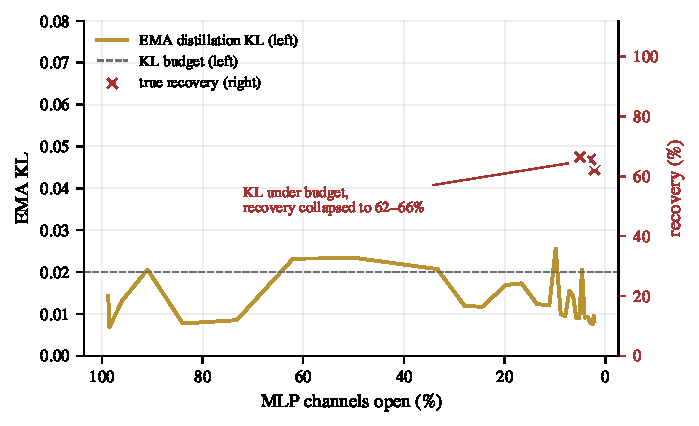
\includegraphics[width=0.58\textwidth]{figures/miscalibration.pdf}
\caption{\textbf{Losses lie; generations don't.} The failed KL-only
controller (v2.0): EMA distillation KL stays under budget throughout the
descent (left axis) while true held-out recovery collapses (crosses, right
axis). Generation probes detect this; losses do not.}
\label{fig:miscal}
\end{figure}

\section{Honest comparison notes}\label{sec:honest}

\begin{itemize}
\item \textbf{Baselines.} Our arithmetic baseline reproduces PRISM's
qualitative finding (attribution masks fail small: 0.3\% recovery at 5\%)
but uses grad$\times$act attribution and zero-isolation rather than their
ReLP and counterfactual patching; PRISM's reported numbers come from their
paper, not our re-runs. Zero-isolation is the harsher operator, so our
baseline understates theirs.
\item \textbf{Function calling.} Comparisons differ in model size (4B vs.\
8B) and metric (verbatim self-match vs.\ BFCL exact match); we present them
as context, not a head-to-head.
\item \textbf{Seeds.} Arithmetic results are 3 seeds; function calling is a
single seed, and its floor was step-cap-limited, not probe-detected.
\item \textbf{Scope.} PRISM's $10^3$ H100-hour budget bought breadth
(translation, an 8B model, extensive controls) that our \$5 did not; the
claim here is that the \emph{per-result} process cost collapses, not that
our evidence is broader.
\end{itemize}

\section{Related work}

PRISM \citep{prism2026} defines the problem, contract, and metric we use;
our method is their stated future direction, built. Learnable $L_0$ masks
during adaptation descend from \citet{louizos2018} and movement pruning
\citep{sanh2020movement}; differentiable circuit discovery applies the same
machinery to interpretability \citep{bhaskar2024edge, conmy2023acdc}. Our
distinction from both is the objective: a behavior-preservation contract
with an unmasked-validity guardrail, rather than aggregate-loss compression
or circuit faithfulness. Self-distillation into a substructure relates to
on-policy and generalized knowledge distillation \citep{hinton2015,
agarwal2024gkd}, here with teacher and student sharing weights and the
student differing only by a mask. Superposition \citep{elhage2022superposition}
explains why attribution-only masks fail and adaptation is necessary; sparse
autoencoders \citep{cunningham2023sae} and weight-sparse training
\citep{gao2025weightsparse} change the basis instead. The lottery-ticket
line \citep{frankle2019lottery} seeks subnetworks that \emph{retrain} to
full performance; extraction requires the behavior to survive \emph{without}
retraining from initialization.

\section{Limitations}

Capabilities are bounded by prompt coverage: the function-calling
generalization gap is a data problem the tool can flag (via held-out
receipts) but not solve. Self-match undercounts semantic fidelity. The
sliced artifact has heterogeneous layer widths and needs a re-slice step on
load. We have not yet run the 8B headline, multi-seed function calling, or
non-Qwen replications beyond CPU-level architecture tests; these are in
progress and gate any stronger claims. Easier extraction also eases misuse
(extracting narrow capabilities from safety-tuned models); receipts and
intended-use documentation ship with the tool, mirroring PRISM's stance.

\section{Conclusion}

PRISM posed capability extraction as a contract---behavior must survive with
the complement switched off---and named training-time budget reshaping as
its highest-value open direction. We built that: one run, on one consumer
GPU, that selects and relocates simultaneously, finds its own floor by
generating rather than by watching losses, and leaves behind a frontier,
integrity receipts, and a model 3.7$\times$ smaller. The headline numbers
surpass the staged pipeline on its own benchmark, but the durable lesson may
be the negative one: logit-level divergence is not behavior, and any metric
built on it will miss collapses that a cheap generation probe catches.
Extraction is now a \texttt{pip install}, not a pipeline.

\section*{Reproducibility}

All numbers in this paper were produced by the released library or the
research scripts in the same repository, on one rented RTX 4090. The paper's
figures regenerate from committed result JSONs via
\texttt{paper/make\_figures.py}.

\bibliographystyle{plainnat}
\bibliography{refs}

\end{document}
